\documentclass[fleqn,10pt]{olplainarticle}
% Use option lineno for line numbers 
\usepackage{url}
\usepackage{graphicx}

\title{Messfehler - M0}

\author[1]{Skopp, Erik}

\author[2]{Skopp, Erik (60XXX) und Treßin, Devin (72XXX)}


\keywords{Messabweichung, Fadenpendel, M0, Grundpraktikum Physik}

\begin{abstract}
In diesem Experiment messen wir die Periodendauer eines Fadenpendels, um die Erdbeschleunigung zu berechnen. Dazu machen wir 200 Messungen und werten sie statistisch aus. Wir lernen, wie man zufällige und systematische Fehler erkennt und die Ergebnisse in Histogrammen darstellt, um den wahren Wert der Periodendauer und die Standardabweichung abzuschätzen..
\end{abstract}
\begin{document}

\flushbottom
\maketitle
\thispagestyle{empty}

\section{Aufgabenstellung}
\begin{enumerate}
    \item Die Periodendauer eines Fadenpendels ist mehrmals zu messen. Die Häufigkeitsverteilung der Messwerte ist in Abhängigkeit von der Anzahl $n$ der Messungen in geeigneten Histogrammen darzustellen. 

    \item Für $n = 200 $ Messwerte sind Schätzwerte für die Standardabweichung $ \sigma $  und den wahren Wert $\mu $ der Messgröße anzugeben und mit grafisch ermittelten Ergebnissen zu vergleichen. 

    \item  Aus Periodendauer und Länge des Pendels ist die Schwerebeschleunigung der Erde einschließlich ihrer kombinierten Unsicherheit zu berechnen. 
\end{enumerate}

\section{Grundlagen}


\section{Versuchsbeschreibung}
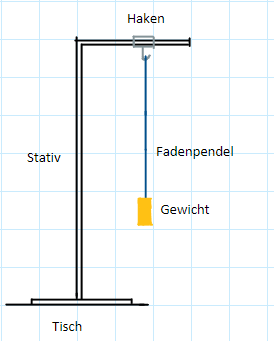
\includegraphics[width=0.5\textwidth]{Messfehler_M0/Experiment.png}



\section{Kontrollfragen}
 \begin{enumerate}
     \item Was versteht man unter einer Messabweichung? In welche beiden Kategorien werden sie unterteilt?
    \begin{enumerate}
     \item \textbf{Messabweichungen}  \\
    Messabweichungen sind unvermeidbare Differenzen in einem Experiment zwischen den gemessenen und den tatsächlichen Werten. Grobe Fehler des Probanten ausgeschlossen, lassen sich Messabweichungen in zwei Kategorien unterteilen. Es ist sehr schwierig, Messfehler vollständig auszuschließen.
        \item \textbf{Zufällige Abweichungen}  \\
        Zufällige Abweichungen sind Messabweichungen die aus einem Experiment nicht auszuschließen sind. Ihnen liegen unkontrollierte Faktoren zugrunde. Daher ist es wichtig ein Experiment nicht nur einmal sondern so oft wie möglich zu wiederholen um auf den genau möglichsten Wert zu kommmen.
        \begin{enumerate}
            \item Menschliche Faktoren. (Ablesefehler, Minimale Fehler bei manuellen Einstellungen)
            \item Unpräzession der Messgeräte. (So liefern bspw alte oder oft benutzte Messgeräte hin und wieder "falsche" oder ungenaue Messwerte)
            \item Äußere Einflüsse. (bspw wenn man "Lüftet und es geht gerade ein Windzug der das Pendel "beschleunigt" oder Aufgrund einer Baustelle nebenan der Boden wackelt)
        \end{enumerate}
        Bei sehr vielen Messungen kann man erkennen, dass diese um den "wahren" Messwert herum pendeln. Daher ist es recht einfach möglich auf den Wahren Wert zu schließen.
        
        \item \textbf{Systematische Abweichungen}  \\
            Systematische Abweichungen sind alle Messabweichungen die sich nicht auf Menschliches Versagen oder die Umwelt zurückzuführen sind. Im Gegensatz zu zufälligen Abweichungen streuen sie nicht um den wahren Wert sondern sind immer systematisch entweder "zu hoch" oder "zu niedrig"  
            \begin{enumerate}
                \item Längenessfehler des Pendels (es kommt zu falschen Werten)
                \item Kalibrierfehler des Messgeräts (Die Zeit könnte zu lang oder zu kurz sein
            \end{enumerate}
    \end{enumerate}
     \item Wie sieht die Dichtefunktion der Normalverteilung aus? Wie sieht das zugehörige Integral aus und was kann man daraus ablesen? 
     \begin{enumerate}
         \item Die Dichtefunktion der Normalverteilung lautet:
                
                \[
                f(x) = \frac{1}{\sigma \sqrt{2\pi}} \exp \left( - \frac{(x - \mu)^2}{2\sigma^2} \right)
                \]
                    \begin{itemize}
        \item \( \mu \) \dots der Erwartungswert (Mittelwert) der Verteilung
        \item \( \sigma \) \dots die Standardabweichung der Verteilung 
    \end{itemize}
     \end{enumerate}
     



     \item Was gibt die Standardabweichung an?  
     \begin{enumerate}
         \item asd
     \end{enumerate}
 \end{enumerate}

\section{Begriffserklärungen}
\begin{enumerate}
    \item Standartabweichung
    \begin{enumerate}
        \item Die Standartabweichung gibt an wie sehr die einzelnen Werte um den Mittelwert schwanken. Je kleiner die Standartabweichung, desto genauer ist der Wert am "wahren" Mittelwert.
    \end{enumerate}

    \item Schwerbeschleunigung der Erde
    \begin{enumerate}
        \item Erdbeschleunigung
        \item Gibt an wie schnell die Geschwindigkeit eines fallenden Objektes im freien Fall zunimmt. 
        \item $g = 9,81\dfrac{m}{s^2}$
    \end{enumerate}
\end{enumerate}


\section{Vorversuch}
Der Vorversuch dient dazu den Hauptversuch besser zu planen und geeignete Intervalle für die Periodendauern festzulegen. 

\section{Versuch}

\end{document}